
%% bare_conf.tex
%% V1.3
%% 2007/01/11
%% by Michael Shell
%% See:
%% http://www.michaelshell.org/
%% for current contact information.
%%
%% This is a skeleton file demonstrating the use of IEEEtran.cls
%% (requires IEEEtran.cls version 1.7 or later) with an IEEE conference paper.
%%
%% Support sites:
%% http://www.michaelshell.org/tex/ieeetran/
%% http://www.ctan.org/tex-archive/macros/latex/contrib/IEEEtran/
%% and
%% http://www.ieee.org/

%%*************************************************************************
%% Legal Notice:
%% This code is offered as-is without any warranty either expressed or
%% implied; without even the implied warranty of MERCHANTABILITY or
%% FITNESS FOR A PARTICULAR PURPOSE! 
%% User assumes all risk.
%% In no event shall IEEE or any contributor to this code be liable for
%% any damages or losses, including, but not limited to, incidental,
%% consequential, or any other damages, resulting from the use or misuse
%% of any information contained here.
%%
%% All comments are the opinions of their respective authors and are not
%% necessarily endorsed by the IEEE.
%%
%% This work is distributed under the LaTeX Project Public License (LPPL)
%% ( http://www.latex-project.org/ ) version 1.3, and may be freely used,
%% distributed and modified. A copy of the LPPL, version 1.3, is included
%% in the base LaTeX documentation of all distributions of LaTeX released
%% 2003/12/01 or later.
%% Retain all contribution notices and credits.
%% ** Modified files should be clearly indicated as such, including  **
%% ** renaming them and changing author support contact information. **
%%
%% File list of work: IEEEtran.cls, IEEEtran_HOWTO.pdf, bare_adv.tex,
%%                    bare_conf.tex, bare_jrnl.tex, bare_jrnl_compsoc.tex
%%*************************************************************************

% *** Authors should verify (and, if needed, correct) their LaTeX system  ***
% *** with the testflow diagnostic prior to trusting their LaTeX platform ***
% *** with production work. IEEE's font choices can trigger bugs that do  ***
% *** not appear when using other class files.                            ***
% The testflow support page is at:
% http://www.michaelshell.org/tex/testflow/



% Note that the a4paper option is mainly intended so that authors in
% countries using A4 can easily print to A4 and see how their papers will
% look in print - the typesetting of the document will not typically be
% affected with changes in paper size (but the bottom and side margins will).
% Use the testflow package mentioned above to verify correct handling of
% both paper sizes by the user's LaTeX system.
%
% Also note that the "draftcls" or "draftclsnofoot", not "draft", option
% should be used if it is desired that the figures are to be displayed in
% draft mode.
%
\documentclass[conference]{IEEEtran}
% Add the compsoc option for Computer Society conferences.
%
% If IEEEtran.cls has not been installed into the LaTeX system files,
% manually specify the path to it like:
% \documentclass[conference]{../sty/IEEEtran}





% Some very useful LaTeX packages include:
% (uncomment the ones you want to load)


% *** MISC UTILITY PACKAGES ***
%
%\usepackage{ifpdf}
% Heiko Oberdiek's ifpdf.sty is very useful if you need conditional
% compilation based on whether the output is pdf or dvi.
% usage:
% \ifpdf
%   % pdf code
% \else
%   % dvi code
% \fi
% The latest version of ifpdf.sty can be obtained from:
% http://www.ctan.org/tex-archive/macros/latex/contrib/oberdiek/
% Also, note that IEEEtran.cls V1.7 and later provides a builtin
% \ifCLASSINFOpdf conditional that works the same way.
% When switching from latex to pdflatex and vice-versa, the compiler may
% have to be run twice to clear warning/error messages.

% *** CITATION PACKAGES ***
%
%\usepackage{cite}
\usepackage{cite}
% cite.sty was written by Donald Arseneau
% V1.6 and later of IEEEtran pre-defines the format of the cite.sty package
% \cite{} output to follow that of IEEE. Loading the cite package will
% result in citation numbers being automatically sorted and properly
% "compressed/ranged". e.g., [1], [9], [2], [7], [5], [6] without using
% cite.sty will become [1], [2], [5]--[7], [9] using cite.sty. cite.sty's
% \cite will automatically add leading space, if needed. Use cite.sty's
% noadjust option (cite.sty V3.8 and later) if you want to turn this off.
% cite.sty is already installed on most LaTeX systems. Be sure and use
% version 4.0 (2003-05-27) and later if using hyperref.sty. cite.sty does
% not currently provide for hyperlinked citations.
% The latest version can be obtained at:
% http://www.ctan.org/tex-archive/macros/latex/contrib/cite/
% The documentation is contained in the cite.sty file itself.






% *** GRAPHICS RELATED PACKAGES ***
%
\ifCLASSINFOpdf
  % \usepackage[pdftex]{graphicx}
  % declare the path(s) where your graphic files are
  % \graphicspath{{../pdf/}{../jpeg/}}
  % and their extensions so you won't have to specify these with
  % every instance of \includegraphics
  % \DeclareGraphicsExtensions{.pdf,.jpeg,.png}
\else
  % or other class option (dvipsone, dvipdf, if not using dvips). graphicx
  % will default to the driver specified in the system graphics.cfg if no
  % driver is specified.
   \usepackage[dvips]{graphicx}
  % declare the path(s) where your graphic files are
   \graphicspath{{../figures/}}
  % and their extensions so you won't have to specify these with
  % every instance of \includegraphics
   \DeclareGraphicsExtensions{.eps}
\fi
% graphicx was written by David Carlisle and Sebastian Rahtz. It is
% required if you want graphics, photos, etc. graphicx.sty is already
% installed on most LaTeX systems. The latest version and documentation can
% be obtained at: 
% http://www.ctan.org/tex-archive/macros/latex/required/graphics/
% Another good source of documentation is "Using Imported Graphics in
% LaTeX2e" by Keith Reckdahl which can be found as epslatex.ps or
% epslatex.pdf at: http://www.ctan.org/tex-archive/info/
%
% latex, and pdflatex in dvi mode, support graphics in encapsulated
% postscript (.eps) format. pdflatex in pdf mode supports graphics
% in .pdf, .jpeg, .png and .mps (metapost) formats. Users should ensure
% that all non-photo figures use a vector format (.eps, .pdf, .mps) and
% not a bitmapped formats (.jpeg, .png). IEEE frowns on bitmapped formats
% which can result in "jaggedy"/blurry rendering of lines and letters as
% well as large increases in file sizes.
%
% You can find documentation about the pdfTeX application at:
% http://www.tug.org/applications/pdftex





% *** MATH PACKAGES ***
%
\usepackage[cmex10]{amsmath}
% A popular package from the American Mathematical Society that provides
% many useful and powerful commands for dealing with mathematics. If using
% it, be sure to load this package with the cmex10 option to ensure that
% only type 1 fonts will utilized at all point sizes. Without this option,
% it is possible that some math symbols, particularly those within
% footnotes, will be rendered in bitmap form which will result in a
% document that can not be IEEE Xplore compliant!
%
% Also, note that the amsmath package sets \interdisplaylinepenalty to 10000
% thus preventing page breaks from occurring within multiline equations. Use:
%\interdisplaylinepenalty=2500
% after loading amsmath to restore such page breaks as IEEEtran.cls normally
% does. amsmath.sty is already installed on most LaTeX systems. The latest
% version and documentation can be obtained at:
% http://www.ctan.org/tex-archive/macros/latex/required/amslatex/math/





% *** SPECIALIZED LIST PACKAGES ***
%
%\usepackage{algorithmic}
% algorithmic.sty was written by Peter Williams and Rogerio Brito.
% This package provides an algorithmic environment fo describing algorithms.
% You can use the algorithmic environment in-text or within a figure
% environment to provide for a floating algorithm. Do NOT use the algorithm
% floating environment provided by algorithm.sty (by the same authors) or
% algorithm2e.sty (by Christophe Fiorio) as IEEE does not use dedicated
% algorithm float types and packages that provide these will not provide
% correct IEEE style captions. The latest version and documentation of
% algorithmic.sty can be obtained at:
% http://www.ctan.org/tex-archive/macros/latex/contrib/algorithms/
% There is also a support site at:
% http://algorithms.berlios.de/index.html
% Also of interest may be the (relatively newer and more customizable)
% algorithmicx.sty package by Szasz Janos:
% http://www.ctan.org/tex-archive/macros/latex/contrib/algorithmicx/




% *** ALIGNMENT PACKAGES ***
%
%\usepackage{array}
% Frank Mittelbach's and David Carlisle's array.sty patches and improves
% the standard LaTeX2e array and tabular environments to provide better
% appearance and additional user controls. As the default LaTeX2e table
% generation code is lacking to the point of almost being broken with
% respect to the quality of the end results, all users are strongly
% advised to use an enhanced (at the very least that provided by array.sty)
% set of table tools. array.sty is already installed on most systems. The
% latest version and documentation can be obtained at:
% http://www.ctan.org/tex-archive/macros/latex/required/tools/


%\usepackage{mdwmath}
%\usepackage{mdwtab}
% Also highly recommended is Mark Wooding's extremely powerful MDW tools,
% especially mdwmath.sty and mdwtab.sty which are used to format equations
% and tables, respectively. The MDWtools set is already installed on most
% LaTeX systems. The lastest version and documentation is available at:
% http://www.ctan.org/tex-archive/macros/latex/contrib/mdwtools/


% IEEEtran contains the IEEEeqnarray family of commands that can be used to
% generate multiline equations as well as matrices, tables, etc., of high
% quality.


%\usepackage{eqparbox}
% Also of notable interest is Scott Pakin's eqparbox package for creating
% (automatically sized) equal width boxes - aka "natural width parboxes".
% Available at:
% http://www.ctan.org/tex-archive/macros/latex/contrib/eqparbox/

\usepackage{tabularx,ragged2e,booktabs}
\DeclareMathSizes{10}{9}{6}{5}
\abovedisplayskip.50ex
\belowdisplayskip.50ex
\abovedisplayshortskip.50ex
\belowdisplayshortskip.50ex
%\restylefloat{figure}
%\restylefloat{table}
%\usepackage{todonotes}
%\usepackage{makeidx}  % allows for indexgeneration
%
\newcolumntype{C}[1]{>{\Centering}m{#1}}
\renewcommand\tabularxcolumn[1]{C{#1}}
\setlength{\parindent}{10pt}
\renewcommand{\tablename}{\bf Table}




% *** SUBFIGURE PACKAGES ***
\usepackage[tight,footnotesize]{subfigure}
% subfigure.sty was written by Steven Douglas Cochran. This package makes it
% easy to put subfigures in your figures. e.g., "Figure 1a and 1b". For IEEE
% work, it is a good idea to load it with the tight package option to reduce
% the amount of white space around the subfigures. subfigure.sty is already
% installed on most LaTeX systems. The latest version and documentation can
% be obtained at:
% http://www.ctan.org/tex-archive/obsolete/macros/latex/contrib/subfigure/
% subfigure.sty has been superceeded by subfig.sty.



%\usepackage{caption}
%\usepackage[font=footnotesize]{subfig}
% subfig.sty, also written by Steven Douglas Cochran, is the modern
% replacement for subfigure.sty. However, subfig.sty requires and
% automatically loads Axel Sommerfeldt's caption.sty which will override
% IEEEtran.cls handling of captions and this will result in nonIEEE style
% figure/table captions. To prevent this problem, be sure and preload
% caption.sty with its "caption=false" package option. This is will preserve
% IEEEtran.cls handing of captions. Version 1.3 (2005/06/28) and later 
% (recommended due to many improvements over 1.2) of subfig.sty supports
% the caption=false option directly:
%\usepackage[caption=false,font=footnotesize]{subfig}
%
% The latest version and documentation can be obtained at:
% http://www.ctan.org/tex-archive/macros/latex/contrib/subfig/
% The latest version and documentation of caption.sty can be obtained at:
% http://www.ctan.org/tex-archive/macros/latex/contrib/caption/




% *** FLOAT PACKAGES ***
%
%\usepackage{fixltx2e}
% fixltx2e, the successor to the earlier fix2col.sty, was written by
% Frank Mittelbach and David Carlisle. This package corrects a few problems
% in the LaTeX2e kernel, the most notable of which is that in current
% LaTeX2e releases, the ordering of single and double column floats is not
% guaranteed to be preserved. Thus, an unpatched LaTeX2e can allow a
% single column figure to be placed prior to an earlier double column
% figure. The latest version and documentation can be found at:
% http://www.ctan.org/tex-archive/macros/latex/base/



\usepackage{stfloats}
% stfloats.sty was written by Sigitas Tolusis. This package gives LaTeX2e
% the ability to do double column floats at the bottom of the page as well
% as the top. (e.g., "\begin{figure*}[!b]" is not normally possible in
% LaTeX2e). It also provides a command:
%\fnbelowfloat
% to enable the placement of footnotes below bottom floats (the standard
% LaTeX2e kernel puts them above bottom floats). This is an invasive package
% which rewrites many portions of the LaTeX2e float routines. It may not work
% with other packages that modify the LaTeX2e float routines. The latest
% version and documentation can be obtained at:
% http://www.ctan.org/tex-archive/macros/latex/contrib/sttools/
% Documentation is contained in the stfloats.sty comments as well as in the
% presfull.pdf file. Do not use the stfloats baselinefloat ability as IEEE
% does not allow \baselineskip to stretch. Authors submitting work to the
% IEEE should note that IEEE rarely uses double column equations and
% that authors should try to avoid such use. Do not be tempted to use the
% cuted.sty or midfloat.sty packages (also by Sigitas Tolusis) as IEEE does
% not format its papers in such ways.





% *** PDF, URL AND HYPERLINK PACKAGES ***
%
%\usepackage{url}
% url.sty was written by Donald Arseneau. It provides better support for
% handling and breaking URLs. url.sty is already installed on most LaTeX
% systems. The latest version can be obtained at:
% http://www.ctan.org/tex-archive/macros/latex/contrib/misc/
% Read the url.sty source comments for usage information. Basically,
% \url{my_url_here}.
%% Package to linebreak URLs in a sane manner.
\usepackage{url}
%% Define a new 'smallurl' style for the package that will use a smaller font.
\makeatletter
\def\url@smallurlstyle{%
  \@ifundefined{selectfont}{\def\UrlFont{\sf}}{\def\UrlFont{\small\ttfamily}}}
\makeatother
%% Now actually use the newly defined style.
\urlstyle{smallurl}
%% Define 'tinyurl' style for even smaller URLs (such as in tables)
\makeatletter
\def\url@tinyurlstyle{%
  \@ifundefined{selectfont}{\def\UrlFont{\sf}}{\def\UrlFont{\scriptsize\ttfamily}}}
\makeatother
\renewcommand{\UrlFont}{\scriptsize}
%
%% Make URLs clickable
\usepackage[colorlinks, bookmarks=false]{hyperref}
%\usepackage{hyperref}
\usepackage{breakurl}
\hypersetup{
    %linktoc=all,     %set to all if you want both sections and subsections linked
    %linkcolor=blue,  %choose some color if you want links to stand out
    colorlinks=false, %set true if you want colored links
    citecolor=black,
    filecolor=black,
    linkcolor=black,
    urlcolor=black
}

%\newcommand\abs[1]{\left|#1\right|}
%
\newcommand{\myfigureshrinker}{\vspace{0.05cm}}
\newcommand{\myfigureshrinkerless}{\vspace{-0.05cm}}
\newcommand{\bibfont}{\small}
%\addtolength{\topmargin}{-9mm}
%\addtolength{\topskip}{-6mm}
\addtolength{\textfloatsep}{-4mm}
\addtolength{\dbltextfloatsep}{-4mm}

%\renewcommand\floatpagefraction{.9}
%\renewcommand\topfraction{.9}
%\renewcommand\bottomfraction{.9}
%\renewcommand\textfraction{.1}   
%\setcounter{totalnumber}{50}
%\setcounter{topnumber}{50}
%\setcounter{bottomnumber}{50}


% *** Do not adjust lengths that control margins, column widths, etc. ***
% *** Do not use packages that alter fonts (such as pslatex).         ***
% There should be no need to do such things with IEEEtran.cls V1.6 and later.
% (Unless specifically asked to do so by the journal or conference you plan
% to submit to, of course. )


% correct bad hyphenation here
\hyphenation{op-tical net-works semi-conduc-tor}


\begin{document}
%
% paper title
% can use linebreaks \\ within to get better formatting as desired
\title{SAX-VSM: \\Interpretable Time Series Classification\\ Using SAX and Vector Space Model}


% author names and affiliations
% use a multiple column layout for up to three different
% affiliations
\author{\IEEEauthorblockN{Pavel Senin}
\IEEEauthorblockA{Information and Computer Sciences Department,\\
University of Hawaii at Manoa, Honolulu, HI, 96822\\
Email: senin@hawaii.edu}
\and
\IEEEauthorblockN{Sergey Malinchik}
\IEEEauthorblockA{Lockheed Martin Advanced Technology Laboratories,\\
3 Executive Campus, Suite 600, Cherry Hill, NJ, 08002\\
Email: sergey.b.malinchik@lmco.com}}

% conference papers do not typically use \thanks and this command
% is locked out in conference mode. If really needed, such as for
% the acknowledgment of grants, issue a \IEEEoverridecommandlockouts
% after \documentclass

% for over three affiliations, or if they all won't fit within the width
% of the page, use this alternative format:
% 
%\author{\IEEEauthorblockN{Michael Shell\IEEEauthorrefmark{1},
%Homer Simpson\IEEEauthorrefmark{2},
%James Kirk\IEEEauthorrefmark{3}, 
%Montgomery Scott\IEEEauthorrefmark{3} and
%Eldon Tyrell\IEEEauthorrefmark{4}}
%\IEEEauthorblockA{\IEEEauthorrefmark{1}School of Electrical and Computer Engineering\\
%Georgia Institute of Technology,
%Atlanta, Georgia 30332--0250\\ Email: see http://www.michaelshell.org/contact.html}
%\IEEEauthorblockA{\IEEEauthorrefmark{2}Twentieth Century Fox, Springfield, USA\\
%Email: homer@thesimpsons.com}
%\IEEEauthorblockA{\IEEEauthorrefmark{3}Starfleet Academy, San Francisco, California 96678-2391\\
%Telephone: (800) 555--1212, Fax: (888) 555--1212}
%\IEEEauthorblockA{\IEEEauthorrefmark{4}Tyrell Inc., 123 Replicant Street, Los Angeles, California 90210--4321}}




% use for special paper notices
%\IEEEspecialpapernotice{(Invited Paper)}




% make the title area
\maketitle


\begin{abstract}
%\boldmath
In this paper, we propose a novel method for characteristic patterns discovery in 
time series. This method, called SAX-VSM, is based on two existing techniques - 
Symbolic Aggregate approXimation and Vector Space Model. SAX-VSM is capable 
to automatically discover and rank time series patterns (features) by their 
“importance” to the class, which not only creates well-performing classifiers
and facilitates clustering, but also provides an interpretable class generalization. 
The accuracy of the method, as shown through experimental evaluation, is at the 
level of the current state of the art. 
While being relatively computationally expensive within a learning phase, 
our method provides fast, precise, and interpretable classification.
\end{abstract}
% IEEEtran.cls defaults to using nonbold math in the Abstract.
% This preserves the distinction between vectors and scalars. However,
% if the conference you are submitting to favors bold math in the abstract,
% then you can use LaTeX's standard command \boldmath at the very start
% of the abstract to achieve this. Many IEEE journals/conferences frown on
% math in the abstract anyway.

% no keywords

% For peer review papers, you can put extra information on the cover
% page as needed:
% \ifCLASSOPTIONpeerreview
% \begin{center} \bfseries EDICS Category: 3-BBND \end{center}
% \fi
%
% For peerreview papers, this IEEEtran command inserts a page break and
% creates the second title. It will be ignored for other modes.
%\IEEEpeerreviewmaketitle

\section{Introduction}
%
Time series classification is an increasingly popular area of the research. 
Within last decades, many time series representations, similarity measures, 
and classification algorithms were proposed \cite{review}. 
These can be divided in two major categories. 
The first category of classification techniques is based on shape-based 
similarity metrics - where distance is measured directly between time series points. 
Classical example of methods from this category is a nearest neighbor (kNN)
classifier built upon Euclidean distance \cite{1NN} or SpADe \cite{spade}. 
The second category consists of classification techniques based on the 
structural similarity metrics which employ some high-level representations 
of time series based on their global or local features. 
Examples from this category include DFT based classifier \cite{DFT}
and bag-of-patterns representation (BOP) \cite{bag_patterns}. 

The development of these two categories can be explained by differences in the 
performance of these techniques. 
While shape-based similarity methods virtually unbeatable on short, 
often pre-processed, time series data \cite{benchmark}, 
they usually fail on long and noisy data sets \cite{indexing},
where structure-based techniques demonstrate a superior performance. 
Furthermore, structure-based methods require less storage space and, usually, 
have a faster classification time, thus, they often implemented in industrial settings. 

Recently, as one of a possible alternatives to this two categories, the time series
shapelets were introduced \cite{shapelet} and gained popularity. A shapelet is a \textit{short 
time series ``snippet''}, that is a representative of class membership. Being exact, this 
approach, potentially, combines the superior precision of shape-based similarity methods, 
and the high-throughput capacity and efficiency of feature-based techniques \cite{logical}. 
However, while demonstrating a superior interpretability, robustness, and similar to kNN algorithms
performance, shapelets-based techniques are quite computationally expensive, which makes 
difficult their adoption for many class classification problems difficult \cite{bagnal}. 

As per current state of the art, it is worth noting, that despite to recent development, to date,
the best algorithm in overall performance is the simple nearest neighbor classifier, that is
accurate and robust \cite{review, benchmark, comparison, classifiers}. Moreover, it depends on a
very few parameters. Nevertheless, while possessing all these qualities, 1NN technique has a n
umber of disadvantages, where the major is that it does not offer any insight into the data, 
while the next is the need for a significantly large training set.

In this work, we propose yet another alternative to 1NN algorithm. Similarly to shapelets, our
technique rests on finding time series subsequences that are characteristic representatives of
a class. However, instead of iterative search for these (as in shapelets case), our algorithm finds 
and ranks by ``importance'' all potential candidate subsequences at once. 
Another difference of proposed algorithm is that it is approximate. Built upon SAX,
which provides smoothing and generalization \cite{sax}, SAX-VSM is able to learn efficiently from a
small training set and handles noisy data effectively. 
All these specificities, in turn, enable precise classification, clustering, and facilitate 
a discovery of characteristic patterns.

\section{Background}
SAX-VSM is based on two well-known techniques. The first technique is 
Symbolic Aggregate approXimation \cite{sax}, which is a high-level symbolic  representation 
of time series data. The second technique is a well known in Information Retrieval (IR) 
Vector Space Model \cite{salton}. 

By utilizing an overlapping sliding window subsequence extraction and SAX, 
our algorithm transforms labeled time series into a single collection of SAX 
words (terms) for each of the training classes - effectively constructing a corpus 
of $N$ documents, where $N$ is a number of classes. 
At the following step, it utilizes \textit{tf$\ast$idf} terms weighting, which results in 
$N$ weight vectors used for SAX-VSM classifier construction. 
Following vector space model, classification procedure relies on cosine similarity metric.

SAX algorithm, however, requires two parameters to be provided as an input, and as per 
today, there is no efficient solution for parameters selection known to the best of our knowledge. 
To solve this problem, we employ a global optimization scheme based on the divided rectangles
(DIRECT) algorithm which does not require any parameters \cite{direct}. DIRECT is a derivative-free
optimization process which possess local and global optimization properties. It converges relatively
quickly and yields a deterministic, optimized solution.

\subsection{Symbolic Aggregate approXimation (SAX)}
Symbolic representation of time series, once introduced \cite{sax}, has attracted much attention by
enabling an application of numerous string-processing algorithms, bioinformatics, and text mining 
tools to temporal data. The method provides a significant reduction of the time series 
dimensionality and a low-bounding to Euclidean distance metric, which guarantees no false 
dismissal \cite{hot_sax}.
These properties are often leveraged by other techniques, which embed SAX representation 
in their algorithms for indexing and approximation. For example, adoption of SAX indexing 
allowed significant shapelets discovery speed improvement in Fast-Shapelets \cite{fast-shapelets}
(but made the algorithm approximate).

%Given a time-series $T$ of a length $n$, SAX produces its symbolic approximation $\hat{S}$ of 
%a length $w$ where letters are taken from an alphabet $\alpha$. 
%Along with $T$, two parameters must be specified as the input: an alphabet size $\alpha$ and 
%a size of the word to produce $w$. Algorithm works as follows. 

%At first, since SAX rests on the assumption that normalized time series tend to have Gaussian 
%distribution \cite{larsen_marx}, the time-series $T$ is normalized to unit of standard deviation
%\cite{goldin_kanellakis}. 
%At the second step, the dimensionality of the normalized time series is reduced to $w$ by 
%obtaining a Piecewise Aggregate Approximation (PAA) of $T$. 
%Specifically, this approximation is obtained by dividing the time series $T$ into $w$ 
%equal-sized segments and computing the mean values for points within each segment. 
%The aggregated sequence of these mean values forms PAA approximation of $T$ of length $w$.
%Finally, each of PAA coefficients is converted into a letter of the alphabet $\alpha$ by the use 
%of lookup tables. These tables are built by defining a set of breakpoints that divide the 
%distribution space into $\alpha$ equiprobable regions \cite{sax}.
Configured by two parameters - a desired word size $w$ and an alphabet size $A$,
SAX produces a symbolic approximation of a time-series $T$ of a length $n$ by compressing 
it into a string of the length $w$ (usually $w<<n$), whose letters are taken from 
the alphabet $\alpha$ ($|\alpha|=A$). 
At the first step of the algorithm, $T$ is z-normalized (to unit of standard deviation)
\cite{goldin_kanellakis}. 
At the second step, a dimensionality of the normalized time series is reduced from $n$ to $w$ by
obtaining its Piecewise Aggregate Approximation (PAA) \cite{paa}; for this, the normalized time
series is
divided into $w$ equal-sized segments and mean values for points within each segment are computed.
The aggregated sequence of these mean values forms PAA approximation of $T$. Finally, each of $w$
PAA coefficients is converted into a letter of an alphabet $\alpha$ by the use of the lookup table.
This table is pre-built by defining a set of breakpoints that divide the normalized time series
distribution 
space into $\alpha$ equiprobable regions. The design of these tables rests on the assumption 
that normalized series tend to have Gaussian distribution \cite{larsen_marx}.

\subsection{Bag of words representation of time series} \label{bow_representation}
Following its introduction, SAX was shown to be an efficient tool for solving problems 
of finding motifs and discords in time series \cite{motifs, hot_sax}. 
The authors employed a sliding window-based subsequence extraction technique 
and augmented data structures (hash table in \cite{motifs} and trie in \cite{hot_sax}) 
in order to build SAX words ``vocabularies''. Further, by analyzing words frequencies 
and locations, they were able to capture frequent and rare SAX words representing 
motifs and discords subsequences. Later, the same technique based on the combination 
of sliding window and SAX was used in the numerous works, most notably in time series 
classification using bag of patterns \cite{bag_patterns}. 

We also use this sliding window technique to convert a time series $T$ of a length $n$ into 
the set of $m$ SAX words, where $m=(n-l_{s})+1$ and $l_{s}$ is the sliding window length. 
By sliding a window of length $l_{s}$ across time series $T$, extracting subsequences, 
converting them to SAX words, and placing these words into an unordered collection, 
we obtain the \textit{bag of words} representation of the original time series $T$.

\subsection{Vector Space Model (VSM) adaptation}
We use Vector space model exactly as it is known in information retrieval (IR) \cite{salton}. 
Similarly to IR, we define and use terms \textit{document}, \textit{bag of words}, 
\textit{corpus}, and \textit{sparse matrix} in our workflow. 
Note however, that we use terms \textit{bag of words} and \textit{document} 
for abbreviation of an unordered collection of SAX words interchangeably, while 
in IR these usually bear different meaning, where a \textit{document} usually 
presumes certain words ordering (semantics). 
Although, similar definitions, such as \textit{bag of features} or 
\textit{bag of patterns}, were previously proposed for techniques built upon 
SAX \cite{bag_patterns}, we use \textit{bag of words} since it reflects our 
workflow precisely. The term \textit{corpus} is used for a structured collection 
of bags of words. 

Given a training set, SAX-VSM builds bags of SAX-generated words representing 
each of the training classes and assembles them into a corpus. 
This corpus, by its construction, is a sparse \textit{term frequency matrix}. 
Rows of this matrix correspond to the set of all SAX words found in 
\textit{all classes}, while each column of the matrix denotes a class of the 
training set. Each element of this matrix is an observed frequency of a word
in a class. 
Many elements of this matrix are zeros - because words extracted from one class 
are often not found in others.
%(Figure \ref{fig:venn}). 
By its design, this sparse 
term frequency matrix is a dictionary of all SAX words extracted from all time 
series of a training set, which accounts for frequencies of each word in each of 
the training classes.

Following to the common in IR workflow, we employ the \textit{tf$\ast$idf} weighting 
scheme for each element of this matrix in order to transform a frequency value into
the weight coefficient. 
The \textit{tf$\ast$idf} weight for a term is defined as a 
product of two factors: term frequency (\textit{tf}) and inverse document 
frequency (\textit{idf}). 
For the first factor, we use logarithmically scaled term frequency \cite{logtf}:
\begin{equation}
 \mbox{tf}_{t, d} =  \begin{cases} \log(1 + \mbox{f}_{t,d}), &\mbox{if f}_{t,d}>0  \\
0, & \mbox{otherwise} \end{cases}
\end{equation} 
where $t$ is the term, $d$ is a bag of words (a \textbf{d}ocument), and $\mbox{f}_{t,d}$ 
is a frequency of the term in a bag.

The inverse document frequency we compute as usual:
\begin{equation}
 \mbox{idf}_{t, D} =  \log_{10}\frac{|D|}{|d \in D : t \in d|} = \log_{10}\frac{N}{\mbox{df}_{t}}
\end{equation} 
where $N$ is the cardinality of corpus $D$ (the total number of classes) and the 
denominator $\mbox{df}_{t}$ is a number of documents where the term $t$ appears.

Then, $\textit{tf$\ast$idf}$ value for a term $t$ in the document $d$ of a corpus $D$ is defined as 
\begin{equation}
 \mbox{tf * idf}(t, d, D) =  \mbox{tf}_{t, d} \times \mbox{idf}_{t, D} = \log(1 + \mbox{f}_{t,d})
\times \log_{10}\frac{N}{\mbox{df}_{t}}
 \label{formula:tfidf}
\end{equation} 
for the all cases where $\mbox{f}_{t,d}>0$ and $\mbox{df}_{t}>0$, or zero otherwise.
Once all terms of a corpus are weighted, the columns of a sparse matrix are used 
as \textit{class term weights vectors} that facilitate the classification using cosine similarity. 

\enlargethispage{0.5cm} 
Cosine similarity measure between two vectors is based on their inner product. 
For two vectors $\boldsymbol{a}$ and $\boldsymbol{b}$ that is:
\begin{equation}
%\mbox{similarity}(\boldsymbol{a},\boldsymbol{b}) = cos(\theta) = \frac{ \sum\limits^{n}_{i=1} a_{i}
%\times b_{i} }{
%\sqrt{\sum\limits^{n}_{i=1} a_{i}} \times \sqrt{\sum\limits^{n}_{i=1} b_{i}} }
\mbox{similarity}(\boldsymbol{a},\boldsymbol{b}) = cos(\theta) = \frac{ 
\mathbf{a} \cdot \mathbf{b} } {\left| \left| a \right| \right| \cdot \left| \left| b \right|
\right|}
\end{equation} 

\subsection{A note on numerosity reduction}
In further SAX development, particularly in its application to problems of discords discovery,
streaming data analyses, and clustering \cite{hot_sax, streaming_sax}, the authors 
proposed a combination of a sampling strategy and a distance function specifically 
designed in order to avoid ``trivial and degenerative solutions''. While the inclusion of
a numerosity reduction was found vital for mentioned applications, intuitively, in our case, 
the over-counting effect is significantly mediated by the design of \textit{tf$\ast$idf}
statistics \eqref{formula:tfidf}. Moreover, by enforcing the exclusion of ``trivial matches'', we
may degrade the overall performance of bag of words based approach, as pointed
in \cite{bag_patterns}.

In order to clarify this issue, we experimented with original combination of a sampling 
strategy and a distance function and found, that for most of the data sets, the inclusion 
of a numerosity reduction significantly reduced DIRECT scheme convergence time 
and improved its accuracy. 
Furthermore, once we relaxed the ``triviality constraints'' by substitution of 
\textit{MINDIST} function \cite{streaming_sax} with Hamming distance \cite{hamming}, 
we were able to improve the classification accuracy for fourteen out of thirty one 
data sets that we have used for the performance evaluation (see \cite{jmotif}).
%
%Thus, we shall explain this in greater detail.
%As noted in \cite{sax}, given a character subsequence $\hat{S_{i}}$ extracted by the use 
%of sliding window and SAX, it is very likely, that $\hat{S_{i}}$ is very similar to its
%neighboring subsequences, $\hat{S_{i-1}}$ and $\hat{S_{i+1}}$ (i.e. those that start one 
%point to the left, and one point to the right of $\hat{S_{i}}$), especially if $\hat{S_{i}}$
%is in the smooth region of the time series - due to the dimensionality reduction. 
%This phenomena results in mapping of multiple consecutive subsequences
%to the same string. The authors called these subsequences as ``trivial matches'' of 
%$\hat{S_{i}}$, and suggested to avoid their over-counting by introducing a 
%``numerosity reduction technique''. This technique is based on the custom distance 
%function \textit{MINDIST} \cite{streaming_sax}, and accounts only for the first 
%occurrence of $\hat{S_{i}}$. 
%
%Similarly to \textit{MINDIST} we define a $dist$ function for two
%SAX words $\hat{Q}$ and $\hat{C}$ as
%\begin{equation}
 %dist(\hat{q_{i}},\hat{c_{i}})=
        %\begin{cases} \qquad  0, & \mbox{, if } | \hat{q_{i}} - \hat{c_{i}} | \leq 1 \\
         %ASCIIdist( \hat{q_{i}} , \hat{c_{i}} ) & \mbox{, otherwise } 
        %\end{cases}
%\end{equation} 
%where $ASCIIdist( \hat{q_{i}}, \hat{c_{i}} )$ is the absolute value of the difference between 
%ASCII codes for letters $\hat{q_{i}}$ and $\hat{c_{i}}$.
%
%By using this function we modified the process a bag of words construction: 
%while sliding a window across a time series and extracting consecutive words
%as explained in Section \ref{bow_representation}, we compare each newly 
%extracted word to the last word added to the bag using $dist$ function. 
%If these words appear to be equal, we discard the new (to be added) word and 
%continue as usual. Since this numerosity reduction strategy is based 
%on previous work we called it $CLASSIC$.
%
%By further experimentation, we discovered, that if we relax this numerosity reduction
%strategy by using Hamming distance \cite{hamming} instead of $dist$ function
%defined above, it is possible to further improve SAX-VSM accuracy for fourteen 
%out of thirty one datasets we used for validation (see \cite{jmotif}). 
%We called this numerosity reduction strategy EXACT, since the use of Hamming 
%distance prevents only exact consecutive trivial matches to be placed into the bag. 

At this point we unable to further comment on these experimental results and 
leaving this phenomenon for the future research.

\section{SAX-VSM classification algorithm }
As many other classification techniques, SAX-VSM consists of two parts - the training
phase, and the classification procedure. In the following sections, we shall explain 
the algorithm in detail, while here, we present an overview of our method 
and outline its specificities and differences from other techniques.

The training of SAX-VSM classifier is relatively computationally expensive 
(Fig. \ref{fig:precision-runtime}) because it involves construction of a corpus by
extraction of SAX words from all labeled series and its post-processing with VSM. 
However, there is no need to maintain an index of training series, or to keep any of 
them in the memory at a runtime: the algorithm simply iterates over all labeled series
incrementally building bags of SAX words for each of the training classes, 
that is, algorithm builds a \textit{single bag of words for each training class}. 
Once built, the corpus of $N$ bags of words (where $N$ is the number of classes) is
processed with \textit{tf$\ast$idf} and can be also discarded - only a resulting set of $N$ 
real-valued weight vectors is retained. 
Note, that the construction of a single bag of words for each of the training classes 
is one of the key differences of SAX-VSM from other previously published 
techniques \cite{bag_patterns}.

The use of cosine similarity for classification is another key difference of SAX-VSM 
from competing techniques. SAX-VSM facilitates a fast classification procedure, 
which consists of the conversion of an unlabeled time series into a terms 
frequency vector, and its successive classification by the computation of $N$ cosine 
values. The unlabeled time series is assigned to a class whose weight vector 
yields a maximal cosine. 

\begin{figure}[t]
   \centering
   \myfigureshrinker
   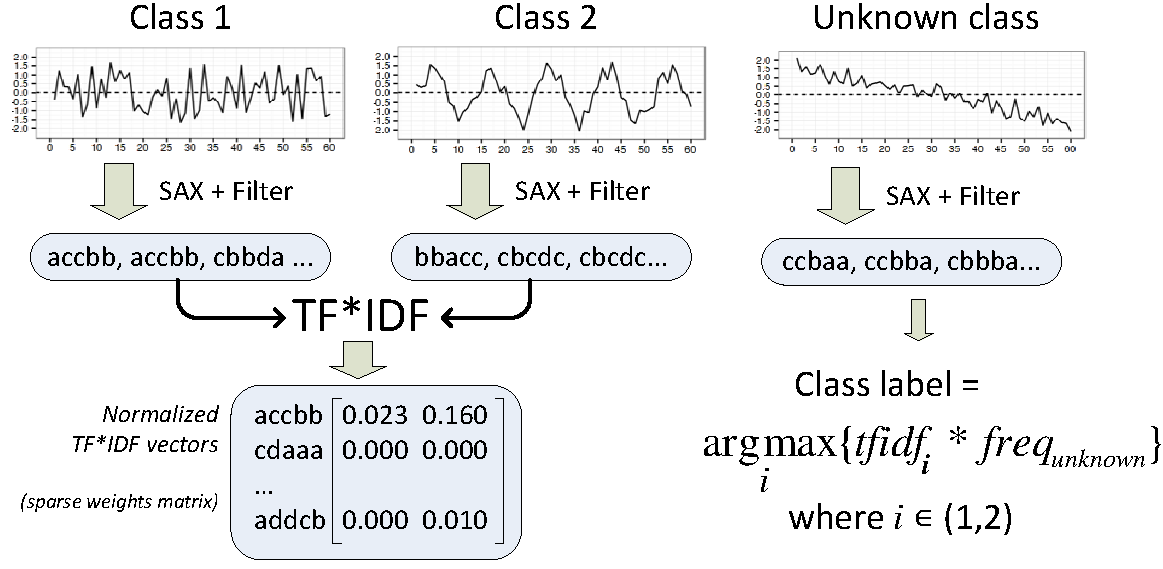
\includegraphics[width=90mm]{figures/overview.eps}
   \caption{
   An overview of SAX-VSM algorithm: 
   at first, labeled time series are converted into bags of words using SAX; 
   secondly, \textit{tf$\ast$idf} statistics is computed resulting in 
   a single weight vector per training class. For classification, an unlabeled 
   time series is converted into a term frequency vector and assigned a 
   label of a weight vector which yields a maximal cosine similarity value.}
   \label{fig:overview}
\end{figure}

\subsection{Training phase}
At first, in order to use Vector space model, algorithm transforms all labeled 
time series into symbolic representation. For this, it converts time series into SAX
representation configured by four parameters: the sliding window length (\textit{W}),
the number of PAA frames per window (\textit{P}), the SAX alphabet size
(\textit{A}), and by the numerosity reduction strategy (\textit{S}). 
As we mentioned, each of the subsequences extracted with sliding window is 
normalized to unit standard deviation before being processed with PAA.
%\cite{goldin_kanellakis}. 
If, however, the standard deviation value falls below a fixed threshold, normalization 
procedure is not applied in order to avoid a possible over-amplification of a low-level 
noise.

By applying this procedure to all $N$ training classes, algorithm builds a corpus 
of $N$ bags, which, in turn, it processes with \textit{tf$\ast$idf}. 
This procedure results in $N$ real-valued weight vectors of equal length 
representing the training classes. 

\subsection{Classification phase}
In order to classify an unlabeled time-series, SAX-VSM transforms it into the 
terms frequency vector using exactly the same sliding window technique and SAX 
parameters that were used within the training phase. 
Then, it computes cosine similarity values between this terms frequency vector and 
$N$ \textit{tf$\ast$idf} weight vectors representing the training classes. 
The unlabeled time series is assigned to the class whose vector yields the maximal 
cosine similarity value.

\begin{figure}[t]
   \myfigureshrinker
   \centering
   \includegraphics[width=90mm]{figures/figure_direct.eps}
   \caption{Parameters optimization with DIRECT for \textit{SyntheticControl} data set. 
   Left panel shows all points sampled by DIRECT in the space $PAA*Window*Alphabet$; here,
   red points correspond to high error values in cross-validation experiments, while green points
   indicate low error values. Note the green points concentration at $W$=42. 
   Middle panel shows an error-rate heat map when the sliding window size is fixed to 42; 
   this figure was obtained by a complete scan of all 432 points of the slice. 
   Right panel shows the optimized by DIRECT sampling. The optimal solution 
   ($W$=42,$P$=8,$A$=4) was found by sampling of 43 points.}
   \label{fig:direct-sampling}
\end{figure}

\subsection{Sliding window size and SAX parameters selection} \label{section-direct}
At this point of SAX-VSM classification algorithm development, it requires a sliding 
window size and SAX parameters to be specified upfront. 
Currently, in order to select optimal parameters values while knowing only a 
training data set, we use a common cross-validation scheme and DIRECT (DIviding RECTangles) 
algorithm, which was introduced in \cite{direct-original}.
However, DIRECT optimization scheme is designed to search for global minima of a real 
valued function over a bound-constrained domain. In order to overcome this limitation, we 
employ the rounding of reported solution values to the nearest integer.

DIRECT algorithm iteratively performs two procedures - partitioning the search domain, 
and identifying potentially optimal hyper-rectangles (i.e., having potential to contain good
solutions). 
It begins by scaling the search domain to a n-dimensional unit hypercube which is considered 
as potentially optimal. The error function is then evaluated at the center of this hypercube. Next, 
other points are created at one-third of the distance from the center in all coordinate directions. 
The hypercube is then divided into smaller rectangles that are identified by their center point 
and their error function value. This procedure continues interactively until error function
converges.
For brevity, we omit the detailed explanation of the algorithm, and refer the 
interested reader to \cite{direct} for additional details. Figure  \ref{fig:direct-sampling} 
illustrates the application of DIRECT to \textit{SyntheticControl} data set.

\subsection{Intuition behind SAX-VSM}
First of all, by combining \textit{\textbf{all}} SAX words observed in \textit{\textbf{all}}
time series of single class into a single bag of words, SAX-VSM manages not only to capture 
observed intraclass variability (as nearest neighbor classifiers), but to efficiently 
``generalize''  it through smoothing capabilities of PAA and SAX.  

Secondly, by partially discarding the original ordering of time series subsequences, and
through subsequence normalization, SAX-VSM is capable to capture and to recognize 
characteristic subsequences in distorted time series (by rotation or shift), as well,
as to recover a signal from corrupted or altered by noise data. 

Thirdly, the \textit{tf$\ast$idf} statistics naturally ``highlights'' terms unique to the
class by assigning them higher weights, while terms observed in multiple classes are 
assigned weights inversely proportional to their interclass presence frequency. 
This weighting scheme improves the selectivity of classification by  lowering the 
contribution of ``confusive'' multi-class terms while increasing  the contribution 
of  class' ``defining'' terms to the final similarity value.   

When combined, these specificities make SAX-VSM time series classification approach 
unique. Ultimately, it compares a set of short overlapping subsequences extracted from a 
full length of an unlabeled time series with a weighted set of all characteristic subsequences
representing a training class.
Thus, an unlabeled time series is classified by its similarity not to a fixed number 
of sequences (as in kNN classifiers), or to a fixed number of characteristic features 
(as in shapelets-based classifiers), but by a product of its subsequences similarity to all 
known subsequences.
This, as we shall show, contributes to the excellent classification performance on temporal 
data sets where time series have a very low intraclass similarity at the full length, but 
embed characteristic to the class subsequences. In particular, note SAX-VSM performance 
on human-driven, aperiodical telemetry stream with a signal loss - ElectricDevices data set
\cite{bagnal} (Table \ref{perf_table}), as well as our previous experimental results on 
software process artifact trails \cite{android}.



\enlargethispage{0.5cm} 
\begin{footnotesize}
\begin{table}[t]
\myfigureshrinkerless
\caption{\bf Classifiers error rates comparison.}
 \label{perf_table}
\centering
\begin{tabularx}{\linewidth}{@{} l *5X @{}}\toprule[1.5pt]
\bf Data set &\bf 1NN-Euclidean &\bf 1NN-DTW &\bf Shapelet Tree &\bf  Shapelet SVM &\bf 
SAX-VSM\\\midrule
%\bf Variable Name & \bf Regression 1 & \bf Mean & \bf Std. Dev & \bf Min & \bf Max\\\midrule
%text        &  text     & text      &  text     &  text     &text\\
%\bottomrule[1.25pt]
%\end {tabularx}
%\begin{tabular}[h]{  l | c | c | c | c |  c  }
%\hline
%Dataset           & 1NN-Euclidean  & 1NN-DTW       & Shapelet Tree & Shapelet SVM & SAX-VSM \\
%\hline
SyntheticControl  & 0.120   & \textbf{0.007}  & 0.057     & 0.127            & 0.010 \\
Adiac             & 0.389   & 0.396           & 0.700        & 0.762         & \textbf{0.381}\\
Beef              & 0.467   & 0.467           & 0.500        & 0.133         & \textbf{0.033}\\
ChlorineConcentration  & 0.350 & 0.350        & 0.412        & 0.439         & \textbf{0.332} \\
Coffee            & 0.250   & 0.180           & 0.036     & \textbf{0.0}     & \textbf{0.0} \\
ECG               & 0.120   & 0.230           & 0.149     & \textbf{0.007}   & 0.09 \\
ElectricDevices   & 0.913   & 0.913           & 0.451     & 0.758            & \textbf{0.329} \\
FaceFour          & 0.216   & 0.170           & 0.159     & 0.023            & \textbf{0.0} \\
Gun Point         & 0.087   & 0.093           & 0.107     & \textbf{0.0}     & 0.007 \\
Lightning7        & 0.425   & \textbf{0.274}  & 0.507     & 0.301            & 0.301 \\
SonyAIBO          & 0.306   & 0.274           & 0.155     & \textbf{0.133}   & 0.176 \\
Trace             & 0.240   & \textbf{0.0}    & 0.020     & 0.020            & \textbf{0.0} \\
\bottomrule[1.25pt]
\end{tabularx}
\end{table}
%\hline
%\end{tabular}
\end{footnotesize}

\section{Results}
We have proposed a novel algorithm for time series classification based on the SAX
representation of time series and Vector Space Model called SAX-VSM. Here, we present 
a range of experiments assessing its performance in classification and clustering.

\subsection{Analysis of classification accuracy}
To evaluate our approach, we selected thirty one data sets. Majority of the data sets was taken 
from the UCR time series repository \cite{ucr}, the Ford data set was downloaded from 
IEEE World Congress on Computational Intelligence \cite{ford} website, the 
ElectricDevices data set was downloaded from supporting website for \cite{bagnal}. 
Overall, SAX-VSM classification performance found to be at the level of best 
performing 1NN classifiers (based on Euclidean distance, DTW, and SAX), 
a shapelet tree, or a shapelet-based SVM. 
This result is not surprising taking in account ``No Free Lunch theorems'' \cite{nfl}, 
which assert, that there will not be a single dominant classifier for all TSC problems.

Table \ref{perf_table} compares the performance of SAX-VSM and four competing 
classifiers: two 1NN classifiers based on Euclidean distance and DTW, 
and two classifiers based on the recently proposed shapelet technique: 
the shapelet decision tree \cite{shapelet, logical}, and 
the best performing shapelet transform classifier based on SVM \cite{bagnal}. 
We selected these particular techniques in order to position SAX-VSM 
in terms of accuracy and interpretability. 
The presented comparison data sets selection is limited to the number 
of previously published benchmark results for all of four competing classifiers. 
The performance of SAX-VSM for the rest of the data sets can be found online 
along with our reference implementation \cite{jmotif}.

In our evaluation, we followed train/test split of the data. We exclusively used train data in 
cross-validation experiments for selection of SAX parameters and numerosity reduction strategy
using DIRECT (Section \ref{section-direct}). Once selected, the optimal set of parameters 
was used to assess SAX-VSM classification accuracy which is reported in the last column 
of the Table \ref{perf_table}.

\begin{figure}[t]
   \myfigureshrinkerless
   \centering
   \includegraphics[width=84mm]{figures/precision-runtime.eps}
   \caption{Comparison of classification precision and runtime of SAX-VSM and 1NN 
   Euclidean classifier on CBF data. SAX-VSM performs significantly better with limited 
   amount of training samples (left panel). While SAX-VSM is faster in time series 
   classification, its performance is comparable to 1NN Euclidean classifier when 
   training time is accounted for (right panel).}
   \label{fig:precision-runtime}
\end{figure}

\subsection{Scalability analysis}
For synthetic data sets, it is possible to create as many instances as one need for experimentation.
We used CBF data set \cite{cbf} to investigate the performance of SAX-VSM and 1NN Euclidean
classifier on increasingly large training data sets of size from ten to a thousand, and a fixed test
data set of ten thousands instances. For small training data sets, SAX-VSM is significantly more
accurate than 1NN Euclidean classifier. However, by the time we had more than 500 time series in
our training set, there was no statistically significant difference in accuracy (Fig.
\ref{fig:precision-runtime}). 
Regarding the runtime cost, due to the comprehensive training, SAX-VSM is more expensive than 
1NN Euclidean classifier on small training sets while more efficient on large sets.
However, SAX-VSM allows to perform training offline and load \textit{tf$\ast$idf} weight vectors
when
needed. If this option utilized, our method performs classification significantly faster than 
1NN Euclidean classifier (Fig. \ref{fig:precision-runtime}).

\subsection{Robustness to noise}
In our experimentation with many data sets, we observed, that the dimensionality of
\textit{tf$\ast$idf} 
weight vectors continues to grow with the growth of the training set size. 
This observation, and the fact that each of SAX words is covering only a short span of a time 
series, prompted the idea that SAX-VSM classifier might be robust to noise and loss of signal.
Intuitively, in such a case, the cosine similarity between high dimensional 
vectors might not degrade significantly enough to cause misclassification.
%While it grows rapidly at the beginning, once
%the dictionary is saturated, growth tend to slow down (left panel of Figure \ref{fig:corrupted}). 
%Nevertheless, by adjusting alphabet and PAA sizes it is possible to keep the number of terms
%significantly large. 

%\begin{figure}[t]
%   \centering
%   \includegraphics[width=120mm]{figures/Venn.eps}
%   \caption{Left panel: illustration of terms growth for CBF corpus and individual classes with 
%   training set size. Right panel: distribution of SAX terms in CBF corpus for training set of 
%   1000 series of each class.}
%   \label{fig:venn}
%\end{figure}
While we plan to perform more exploration, current experimentation with CBF data set revealed 
promising results. 
In one series of experiments, by fixing a training set size to two hundred fifty time series, we
varied the standard deviation of Gaussian noise in CBF model (whose default value is about 
17\% of a signal level). SAX-VSM increasingly outperformed 1NN Euclidean classifier 
with the growth of a noise level (Fig.\ref{fig:corrupted} Left). 
Further improvement of SAX-VSM performance was achieved by proportionally increasing
the size of SAX sliding window following the noise growth (Fig.\ref{fig:corrupted}
Left, \textit{SAX-VSM Opt} curve). 
In another series of experiments, we randomly replaced up to fifty percent of a span of unlabeled
time series with a random noise. Again, SAX-VSM performed consistently better than 
1NN Euclidean classifier regardless of a training set size, which we varied from five to
one thousand. The \textit{SAX-VSM Opt} curve at Fig.\ref{fig:corrupted} (Right) depicts the case
with fifty training series when the sliding window size was decreased inversely proportionally 
to the growth of a signal loss.

\begin{figure}[t]
  \myfigureshrinkerless
  \centering
  \includegraphics[width=84mm]{figures/corrupted.eps}
  \caption{Classification performance with presence of noise
 (left panel; the noise level varies up to 100\% of standard deviation(???) ), and with signal loss
(right panel). \textit{SAX-VSM Opt} curves correspond to 
 results obtained with ``optimized''  for each case SAX parameters.}
  \label{fig:corrupted}
\end{figure}

\subsection{Exploratory data analysis}
While the classification performance results in previous sections show that SAX-VSM 
classifier has a very good potential, its major strength is in the level of allowed 
interpretability of classification results. Which, in fact, was our main motivation for this 
work - to design a classification technique that is not only accurate and reliable, but 
also highly interpretable, thus can be applicable to the problem of discovery of 
unknown behaviors \cite{android}.

Previously, in original shapelets work \cite{shapelet, logical}, it was shown that the 
resulting decision trees provide interpretable classification and offer an insight into the data
specific features. In successive work based on shapelets \cite{bagnal}, it was shown that
the discovery of multiple shapelets provides much better resolution and intuition into 
the interpretability of classification. 
However, as the authors noted, a time cost of multiple shapelets discovery
in many class problems could be very significant. Contrary, SAX-VSM extracts and weights 
all patterns at once, without any added cost. Thus, it could be the only choice for interpretable 
classification in many class problems.

\begin{figure}[t]
   \myfigureshrinker
   \centering
   \includegraphics[width=87mm]{figures/gun-point.eps}
   \caption{Best characteristic subsequences discovered by SAX-VSM in \textit{Gun/Point}
   data set. 
   Left panel shows actor's stills and time series annotations made by an expert, 
   right panels show (bold lines) locations of characteristic subsequences.
   Note, that while the upward arm motion found more ``important'' in \textit{Gun} 
   class (gun retrieval and aiming), the downward arm motion better characterizes 
   \textit{Point} class (an ``overshoot'' phenomena in propless arm return). 
   This result aligns with previous work \cite{shapelet} and \cite{bagnal}.
   (Stills and annotation used with permission from E. Keogh) }
   \label{fig:shapelet-like-patterns}
\end{figure}

\subsubsection{Gun Point data set}
Following previously mentioned shapelet-based work \cite{shapelet, bagnal}, 
we used a well-studied \textit{GunPoint} data set \cite{gun} to explore the 
interpretability of classification results. This data set contains two classes: 
time-series in \textit{Gun} class correspond to the actors' hands motion when drawing
a replicate gun from a hip-mounted holster, pointing it at a target for a second,
and returning the gun to the holster; 
time-series in \textit{Point} class correspond to the actors hands motion when pretending
of drawing a gun - the actors point their index fingers to a target for about a second, 
and then return their hands to their sides. 

Similarly to previously reported results \cite{shapelet, bagnal}, 
SAX-VSM was able to capture all distinguishing features as shown at the 
Figure \ref{fig:shapelet-like-patterns}. The most weighted by SAX-VSM patterns in 
\textit{Gun} class corresponds to fine extra movements required to lift and aim the prop. 
The most weighted SAX pattern in \textit{Point} class corresponds to the ``overshoot''
phenomena which is causing the dip in the time series. 
Also, similarly to the original work \cite{gun}, SAX-VSM highlighted as second to the best
patterns in \textit{Point} class the lack of distinguishing subtle extra movements required
for lifting a hand above a holster and reaching down for the gun.

\begin{figure}[t]
   \myfigureshrinker
   \centering
   \includegraphics[width=87mm]{figures/AcerCircunatum.eps}
   \caption{Best characteristic subsequences discovered by SAX-VSM in \textit{OSULeaf data set}.
These patterns align with well known in botany discrimination techniques
by lobe shapes, serrations, and leaf tip types \cite{dirr}.}
   \label{fig:shapelet-acer-patterns}
\end{figure}

\subsubsection{OSU Leaf data set}
According to the original data source, Ashid Grandhi \cite{osuleaf}, with the current growth of
digitized data, there is a huge demand for automatic management and retrieval of various images. The
\textit{OSULeaf} data set consist of curves obtained by color image segmentation and boundary
extraction (in the anti-clockwise direction) from digitized leaf images of six classes: \textit{Acer
Circinatum, Acer Glabrum, Acer Macrophyllum, Acer Negundo, Quercus Garryana and Quercus Kelloggii}.
The authors were able to solve the problem of leaf boundary curves classification by use of DTW, 
achieving 61\% of classification accuracy. However, as we pointed above, DTW provided a
very little information about why it succeeded of failed. 

In contrast, SAX-VSM application yielded a set of class-specific characteristic patterns for each of
six leaves classes from \textit{OSULeaf} data set. These characteristic patterns closely match
known techniques of leaves classification based on leaf shape and margin \cite{dirr}. 
Highlighted by SAX-CSM features include the slightly lobed shape and acute tips of
Acer Circinatum leaves, serrated blade of Acer Glabrum leaves, the acuminate tip and characteristic
serration of in Acer Macrophyllum leaves, pinnately compound leaves arrangement of Acer Negundo, the
incised leaf margin of Quercus Kelloggii, and a lobed leaf structure of Quercus Garryana. 
Figure \ref{fig:shapelet-acer-patterns} shows a subset of these characteristic patterns and original
leaf images with highlighted corresponding features.

\subsubsection{Coffee data set}
Another illustration of interpretable classification with SAX-VSM is based on the analysis of its
performance on Coffee dataset \cite{coffee}. The curves in this dataset correspond to spectra
obtained with diffuse reflection infrared Fourier transform (DRIFT) and truncated to 286 data points
in the region 800-1900 cm$^{-1}$. The two top-ranked by SAX-VSM subsequences in both datasets
correpond to spectrogram intervals of Chlorogenic acid (best) and Caffeine (second to best).
These two chemical compounds are known to be responsible for the flavor differences in 
Arabica and Robusta coffees; moreover, these spectrogram intervals were reported 
as discriminative when used in PCA-based technique by the authors of the original work
\cite{coffee}.

\begin{figure}[t]
   \myfigureshrinker
   \centering
   \includegraphics[width=84mm]{figures/coffee_patterns.ps}
   \caption{Best characteristic subsequences discovered by SAX-VSM in \textit{Coffee data set}.
   The best subsequences in both classes correspond to chlorogenic acid, while
   second to best subsequences - to caffeine. This result aligns with previous 
   exploratory research based on PCA \cite{coffee}.}
   \label{fig:coffee}
\end{figure}

\section{Clustering}
Clustering is a common tool used for data partitioning, visualization, exploration, and serves as
an important subroutine in many data mining algorithms. Typically, clustering algorithms
are built upon a distance function, and the overall performance of an algorithm is highly
dependent on the performance of the chosen function. Thus, an experimental evaluation of the 
proposed technique in clustering provides an additional perspective on its performance and
applicability beyond the classification.

\subsection{Hierarchical clustering}
Probably, one of the most used clustering algorithms is hierarchical clustering which requires no
parameters to be specified \cite{hcs}. It computes pairwise distances between all objects and 
produces a nested hierarchy of clusters offering a great data visualization power. 

Previously, it was shown that the bag-of-patterns time series representation and Euclidean distance
provide a superior clustering performance\cite{bag_patterns}. 
For comparison, we performed similar experiments which differ in time series representation and
distance metric - we relied on \textit{tf$\ast$idf} weight vectors and cosine similarity. 
Affirming the previous work, we found, that the combination of SAX and Vector space model
outperforms classical shape-based distance metrics. 
For example, figure \ref{fig:hc} depicts the result of hierarchical clustering of a subset of
\textit{SyntheticControl} data. 
As one can see, SAX-VSM is superior in clustering performance to Euclidean and DTW distance 
metrics in this particular setup - it produced a hierarchy which properly partitions the
data set into three branches.

\subsection{k-Means clustering}
Another popular choice for data partitioning is k-Means clustering algorithm \cite{kmeans}.
The basic intuition behind this algorithm is that through the iterative reassignment of objects 
into different clusters the intra-cluster distance is minimized. As was shown, k-Means 
algorithm scales much better than hierarchical partitioning techniques \cite{kscale}.
Fortunately, this clustering technique is well studied in IR field. Previously, in \cite{zhao}, the
authors extensively examined seven different criterion functions for partitional document
clustering and found, that \textit{k}-prototypes partitioning with cosine dissimilarity delivers an
excellent performance. 

Following this work, we implemented a similar to \cite{modha} \textit{spherical k-means algorithm}
and found, that algorithm converges quickly and delivers a satisfactory partitioning on short
synthetic data sets. Further, we evaluated our technique on the long time series from PhysioNet 
archive \cite{physionet}. 
We extracted two hundred fifty series corresponding to five vital signals: two ECG leads 
(aVR and II), and RESP, PLETH, and CO2 waves, trimming them to 2'048 points. Similarly to
\cite{bag_patterns}, we run a reference k-Means algorithm implementation based on Euclidean
distance, which achieved the maximum clustering quality of 0.39, when measured as proposed in
\cite{kmetrics} on the best clustering (the one with the smallest objective function in 10 runs). 
SAX-VSM spherical k-Means implementation outperformed the reference technique yielding 
clusters  with the quality of 0.67 (on 10 runs with SAX parameters set of 
$W$=33, $P$=8, $A$=6).

Note also, that previously, we applied our implementation to recurrent behaviors (motifs) 
discovery in software development telemetry streams\cite{android}. 
These behavioral time series were extracted from software change repositories and are 
structurally similar to \textit{ElectricDevices} data set. 
We used our \textit{tf$\ast$idf} weight vectors time series representation and spherical 
k-Means implementation in order to discover specific temporal features corresponding 
to the software release cycle. 
Specifically, we optimized SAX parameters in order to obtain a proper partitioning of known 
development behaviors before and after the software release. 
In turn, the centroids of these clusters represented by \textit{tf$\ast$idf} weight vectors 
were used to classify unlabeled  temporal intervals. 
This technique allowed us to successfully classify pre- and post-release
behaviors with accuracy above 80\%.

\begin{figure}[t]
   \myfigureshrinker
   \centering
   \includegraphics[width=87mm]{figures/clustering.eps}
   \caption{An comparison of hierarchical clustering application to a subset of three
   \textit{SyntheticControl} classes: \textit{Normal, Decreasing trend}, and \textit{Upward shift}. 
   Euclidean distance, Dynamic time warping, SAX-VSM and Complete linkage were used to 
   generate these plots. Only SAX-VSM was able to partition series properly.                       
   }
   \label{fig:hc}
\end{figure}

\section{Conclusion and Future Work}
In this paper, we have proposed a novel interpretable technique for time series classification
based on characteristic patterns discovery. We have shown, that our approach is competitive with, 
or superior to, other techniques on a variety of classic data mining problems. In addition, 
we described several advantages of SAX-VSM over existing structure-based similarity measures,
emphasizing its capacity to discover and rank short subsequences by their class characterization
power.

The current limitations of our SAX-VSM implementation suggest a number of future work directions. 
First of all, while Vector space model naturally supports processing of bags of words composed 
of terms of variable length, our current ``stable'' implementation lacks this capacity.
Inspired by the recently reported superior performance of multi-shapelets based classifiers
\cite{bagnal}, we prioritize this development.
Secondly, while DIRECT optimization provides satisfactory performance, it is designed for a 
function of a real variable. By using rounding in our implementation, we have observed DIRECT 
iteratively sampling redundant locations in suboptimal neighborhood, thus, a more appropriate 
optimization scheme is needed.
Finally, we are designing and experimenting with an extension of SAX-VSM to multidimensional time
series. Currently we are evaluating two candidate implementations: the first is based on a
single bag of words accommodating all dimensions for a class (by prefixing SAX words extracted from
different dimensions); while the second is based on the use of a single bag of words per each of
dimensions. The preliminary results on synthetic data sets look promising and we expect to report 
our finding soon.

% An example of a floating figure using the graphicx package.
% Note that \label must occur AFTER (or within) \caption.
% For figures, \caption should occur after the \includegraphics.
% Note that IEEEtran v1.7 and later has special internal code that
% is designed to preserve the operation of \label within \caption
% even when the captionsoff option is in effect. However, because
% of issues like this, it may be the safest practice to put all your
% \label just after \caption rather than within \caption{}.
%
% Reminder: the "draftcls" or "draftclsnofoot", not "draft", class
% option should be used if it is desired that the figures are to be
% displayed while in draft mode.
%
%\begin{figure}[!t]
%\centering
%\includegraphics[width=2.5in]{myfigure}
% where an .eps filename suffix will be assumed under latex, 
% and a .pdf suffix will be assumed for pdflatex; or what has been declared
% via \DeclareGraphicsExtensions.
%\caption{Simulation Results}
%\label{fig_sim}
%\end{figure}

% Note that IEEE typically puts floats only at the top, even when this
% results in a large percentage of a column being occupied by floats.


% An example of a double column floating figure using two subfigures.
% (The subfig.sty package must be loaded for this to work.)
% The subfigure \label commands are set within each subfloat command, the
% \label for the overall figure must come after \caption.
% \hfil must be used as a separator to get equal spacing.
% The subfigure.sty package works much the same way, except \subfigure is
% used instead of \subfloat.
%
%\begin{figure*}[!t]
%\centerline{\subfloat[Case I]\includegraphics[width=2.5in]{subfigcase1}%
%\label{fig_first_case}}
%\hfil
%\subfloat[Case II]{\includegraphics[width=2.5in]{subfigcase2}%
%\label{fig_second_case}}}
%\caption{Simulation results}
%\label{fig_sim}
%\end{figure*}
%
% Note that often IEEE papers with subfigures do not employ subfigure
% captions (using the optional argument to \subfloat), but instead will
% reference/describe all of them (a), (b), etc., within the main caption.


% An example of a floating table. Note that, for IEEE style tables, the 
% \caption command should come BEFORE the table. Table text will default to
% \footnotesize as IEEE normally uses this smaller font for tables.
% The \label must come after \caption as always.
%
%\begin{table}[!t]
%% increase table row spacing, adjust to taste
%\renewcommand{\arraystretch}{1.3}
% if using array.sty, it might be a good idea to tweak the value of
% \extrarowheight as needed to properly center the text within the cells
%\caption{An Example of a Table}
%\label{table_example}
%\centering
%% Some packages, such as MDW tools, offer better commands for making tables
%% than the plain LaTeX2e tabular which is used here.
%\begin{tabular}{|c||c|}
%\hline
%One & Two\\
%\hline
%Three & Four\\
%\hline
%\end{tabular}
%\end{table}


% Note that IEEE does not put floats in the very first column - or typically
% anywhere on the first page for that matter. Also, in-text middle ("here")
% positioning is not used. Most IEEE journals/conferences use top floats
% exclusively. Note that, LaTeX2e, unlike IEEE journals/conferences, places
% footnotes above bottom floats. This can be corrected via the \fnbelowfloat
% command of the stfloats package.



%\section{Conclusion}
%The conclusion goes here.




% conference papers do not normally have an appendix


% use section* for acknowledgement
%\section*{Acknowledgment}


%The authors would like to thank...





% trigger a \newpage just before the given reference
% number - used to balance the columns on the last page
% adjust value as needed - may need to be readjusted if
% the document is modified later
%\IEEEtriggeratref{8}
% The "triggered" command can be changed if desired:
%\IEEEtriggercmd{\enlargethispage{-5in}}

% references section

% can use a bibliography generated by BibTeX as a .bbl file
% BibTeX documentation can be easily obtained at:
% http://www.ctan.org/tex-archive/biblio/bibtex/contrib/doc/
% The IEEEtran BibTeX style support page is at:
% http://www.michaelshell.org/tex/ieeetran/bibtex/
\bibliographystyle{IEEEtran}
% argument is your BibTeX string definitions and bibliography database(s)
%\bibliography{IEEEabrv,../bib/paper}
%
% <OR> manually copy in the resultant .bbl file
% set second argument of \begin to the number of references
% (used to reserve space for the reference number labels box)
\begin{thebibliography}{5}
%1
\bibitem {review}
Wang, X., Mueen, A., Ding, H., Trajcevski, G., Scheuermann, P., Keogh, E.:
Experimental comparison of representation methods and distance measures for time series data.
Data Min. Knowl. Discov., 26, 2, 275--309 (2013)

%2
\bibitem {1NN}
Xi, X., Keogh, E., Shelton, C., Wei, L., Ratanamahatana, C.:
Fast time series classification using numerosity reduction. 
In Proc. ICML, 1033--1040 (2006)

%3
\bibitem {spade}
Chen, Y., Chen, K., Nascimento, M.:
Effective and Efficient Shape-Based Pattern Detection over Streaming Time Series. 
IEEE TKDE, 265--278 (2012)

%4
\bibitem {DFT}
Agrawal, R., Faloutsos, C., Swami, A.:
Efficient Similarity Search In Sequence Databases.
In Proc. FODO, 69--84 (1993)

%5
\bibitem {bag_patterns}
Lin, J., Khade, R., Li, Y.:
Rotation-invariant similarity in time series using bag-of-patterns representation. 
J. Intell. Inf. Syst. 39, 2, 287--315 (2012)

%6
\bibitem {benchmark}
Keogh, E., Kasetty, S.:
On the need for Time Series Data Mining Benchmarks: a survey and empirical demonstration.
In Proc. ACM DMKD, 102--111 (2002)

%7
\bibitem {indexing}
Keogh, E.:
Exact indexing of dynamic time warping. 
In Proc. VLDB, 406--417 (2002)

%8
\bibitem {shapelet}
Ye, L., Keogh, E.:
Time series shapelets: a novel technique that allows accurate, interpretable and fast
classification.
Data Min. Knowl. Discov.,  149-182, (2011)

%9
\bibitem {logical}
Mueen, A., Keogh, E., Young, N.:
Logical-shapelets: an expressive primitive for time series classification.
In Proc. 17th ACM SIGKDD, 1154--1162 (2011)

%10
\bibitem {bagnal}
Lines, J., Davis, L., Hills, J., Bagnall, A.:
A shapelet transform for time series classification. 
In Proc. 18th ACM SIGKDD, 289--297 (2012)

%11
\bibitem {comparison}
Ding, H., Trajcevski, G., Scheuermann, P., Wang, X., Keogh, E.:
Querying and Mining of Time Series Data: Experimental Comparison of Representations and Distance
Measures. 
In Proc. the 34th VLDB, 1542--1552 (2008)

%12
\bibitem {classifiers}
Salzberg, S.:
On comparing classifiers: Pitfalls to avoid and a recommended approach. 
Data Min. Knowl. Discov., 1, 317--328 (1997)

%13
\bibitem {sax}
Lin, J., Keogh, E., Wei, L., Lonardi, S.:
Experiencing SAX: a novel symbolic representation of time series.
Data Min. Knowl. Discov., 107--144 (2007)

%14
\bibitem {salton}
Salton, G., Wong, A., Yang., C.:
A vector space model for automatic indexing. 
Commun. ACM 18, 11, 613--620 (1975)

%15
\bibitem {direct}
Bj\"{o}rkman, M., Holmstr\"{o}m, K.:
Global Optimization Using the DIRECT Algorithm in Matlab.
Advanced Modeling and Optimization, 1(2), 17--37 (1999)

%16
\bibitem {hot_sax}
Keogh, E., Lin, J., Fu, A.:
HOT SAX: Efficiently Finding the Most Unusual Time Series Subsequence. 
In Proc. ICDM. 226--233 (2005)

%17
\bibitem {fast-shapelets}
Rakthanamanon, T., Keogh, E.:
Fast-Shapelets: A Scalable Algorithm for Discovering Time Series Shapelets.
In Proc. SDM (2013)

%18
\bibitem {goldin_kanellakis}
Goldin D., Kanellakis, P.:
On Similarity Queries for Time-Series Data: Constraint Specification and Implementation. 
In Proc CP. 137--153 (1995)

%not used
\bibitem {paa}
Keogh, E., Pazzani, M.:
A Simple Dimensionality Reduction Technique for Fast Similarity Search in Large Time Series
Databases. In Proc. PADKK, 122--133 (2000)

%19
\bibitem {larsen_marx}
Larsen, R., Marx, M.:
An Introduction to Mathematical Statistics and Its Applications, (3rd Ed.),
Prentice Hall (2000)

%20
\bibitem {motifs}
Chiu, B., Keogh, E., Lonardi, S.:
Probabilistic discovery of time series motifs. 
In Proc. 9th ACM SIGKDD (2003)

\bibitem {logtf}
Manning, C., Raghavan, P., Sch\"utze, H.: 
Introduction to Information Retrieval, Cambridge University Press (2008)

%21
\bibitem {streaming_sax}
Lin, J., Keogh, E., Lonardi, S., Chiu, B.:
A symbolic representation of time series, with implications for streaming algorithms. 
In Proc. 8th DMKD. 2--11 (2003)

%22
\bibitem {hamming}
Hamming, R.:
Error detecting and error correcting codes. 
Bell System Technical Journal 29, pp. 147--160 (1950)

%23
\bibitem {jmotif}
Paper Authors:
Accompanying information for this paper. 
\url{https://code.google.com/p/jmotif/}

%24
\bibitem {direct-original}
Jones, D., Perttunen, C., Stuckman, B.:
Lipschitzian Optimization without Lipschitz Constant.
J. Optim. Theory Appl. 79, 1 (1993)

%25
\bibitem {ucr}
Keogh, E., Zhu, Q., Hu, B., Hao, Y.,  Xi, X., Wei, L., Ratanamahatana, C.:
The UCR Time Series Classification/Clustering Homepage:
\url{http://www.cs.ucr.edu/~eamonn/time_series_data/}

%26
\bibitem {ford}
WCCI, Ford classification challenge,
\url{http://home.comcast.net/~nn_classification/}

%27
\bibitem {nfl}
Wolpert, D., Macready, W.:
No free lunch theorems for optimization.
IEEE Trans. on Evo. Comp. 1 no. 1, 67--82 (1997)

%28
\bibitem {cbf}
Saito, N:
Local feature extraction and its application using a library of bases. 
PhD thesis, Yale University (1994)

%38
\bibitem {android}
Senin, P.: 
Recognizing recurrent development behaviors corresponding to Android OS release life-cycle.
In Proc. SERP (2012)

%29
\bibitem {gun}
Ratanamahatana, C., Keogh, E.:
Making time-series classification more accurate using learned constraints. 
In SDM '04 (2004)

%30
\bibitem {osuleaf}
Gandhi, A.:
Content-Based Image Retrieval: Plant Species Identification. 
MS thesis, Oregon State University (2002)

%31
\bibitem {dirr}
Dirr, M.:
Manual of Woody Landscape Plants: Their Identification, Ornamental Characteristics,
Culture, Propogation and Uses.
Stipes Pub Llc, ed. 6 Revised (2009)

%32
\bibitem {coffee}
Briandet, R., Kemsley, E., Wilson, R.:
Discrimination of Arabica and Robusta in Instant Coffee by Fourier Transform Infrared Spectroscopy
and Chemometrics.
J. Agric. Food Chem, 44, 170--174 (1996)

%33
\bibitem {hcs}
Johnson, C.:
Hierarchical clustering schemes.
Psychometrika, 32(3), 241--254 (1967)

%34
\bibitem {kmeans}
MacQueen, J.:
Some methods for classification and analysis of multivariate observations
Proc. of 5th Berkeley Symp. On  Math. Stat. and Prob., 1, 281--296 (1967)

%35
\bibitem {kscale}
Bradley, P., Fayyad, U., Reina, C.:
Scaling clustering algorithms to large databases. 
In Proc. KDD, 9--15 (1998)

\enlargethispage{0.5cm} 
%36
\bibitem {zhao}
Zhao, Y., Karypis, G.:
Empirical and Theoretical Comparisons of Selected Criterion Functions for Document Clustering.
Mach. Learn., 55, 311--331 (2004)

%37
\bibitem {modha}
Dhillon, I., Modha, D.:
Concept Decompositions for Large Sparse Text Data Using Clustering.
Mach. Learn., 42(1), 143--175 (2001)

\bibitem {physionet}
Goldberger, A., Amaral, L., Glass, L., et al.: PhysioBank, PhysioToolkit, and 
PhysioNet: Circulation. Discovery 101(23), 1(3), 215--220 (1997) 

\bibitem {kmetrics}
Gavrilov, M., Anguelov, D., Indyk, P., Motwani, R.:
Mining the stock market: which measure is best? 
In Proc. 6th KDD. 487--496 (2000)
\end{thebibliography}




% that's all folks
\end{document}


